%
% Exemplo LaTeX de artigo UNISINOS
%
% Elaborado com base nas orientações dadas no documento
% ``GUIA PARA ELABORAÇÃO DE TRABALHOS ACADÊMICOS''
% disponível no site da biblioteca da Unisinos.
% http://www.unisinos.br/biblioteca
%
% Os elementos textuais abaixo são apresentados na ordem em que devem
% aparecer no documento.  Repare que nem todos são obrigatórios - isso
% é devidamente indicado em cada caso.
%
% Comentários abaixo colocados entre aspas (`` '') foram
% extraídos diretamente do documento da biblioteca.
%
% Este documento é de domínio público.
%

%=======================================================================
% Declarações iniciais identificando a classe de documento e
% selecionando alguns pacotes adicionais.
%
% As opções disponíveis (separe-as com vírgulas, sem espaço) são:
% - twoside: Formata o documento para impressão frente-e-verso
%   (o default é somente-frente)
% - english,brazilian,french,german,etc.: idiomas usados no documento.
%   Deve ser colocado por último o idioma principal.
%=======================================================================
\documentclass[twoside,english,brazilian]{UNISINOSartigo}
\usepackage[utf8]{inputenc} % charset do texto (utf8, latin1, etc.)
\usepackage[T1]{fontenc} % encoding da fonte (afeta a sep. de sílabas)
\usepackage{graphicx} % comandos para gráficos e inclusão de figuras
\usepackage{bibentry} % para inserir refs. bib. no meio do texto

%=======================================================================
% Escolha do sistema para geração de referências bibliográficas.
%
% O default é usar o estilo unisinos.bst.  Comente a definição abaixo
% e descomente a linha seguinte para usar o estilo do ABNTeX (é
% necessário ter esse pacote instalado).
%
% A vantagem do unisinos.bst é que ele permite o uso de um arquivo .bib
% seguindo as orientações tradicionais do BibTeX (veja essas orientações
% em http://ctan.tug.org/tex-archive/biblio/bibtex/contrib/doc/btxdoc.pdf).
% Entretanto, o estilo não suporta algumas citações mais exóticas como
% apud.  Para isso, use o ABNTeX, mas esteja ciente de que muitas de
% suas referências serão incompatíveis com os estilos tradicionais do
% BibTeX como plain, alpha, ieeetr, entre outros.
%=======================================================================
\unisinosbst
%\usepackage[alf]{abntcite}

%=======================================================================
% Informações Pessoais
%=======================================================================
\title{Proposta de gamificação nos testes de software}

\author{Cássio Linden Albert}
\authorinfo{Aluno do curso de Sistemas de Informação. Email: cassiola@edu.unisinos.br}
\degree{Bacharel em Sistemas de Informação}
\course{Curso de Sistemas de Informação}
\address{São Leopoldo}
\date{2019}

\advisor{Cristiano Bonato Both}
% [Prof. Dr.]
\advisorinfo{Professor da Unisinos. Email: cboth@unisinos.br}

%=======================================================================
% Início do documento.
%=======================================================================
\begin{document}

\maketitle

%=======================================================================
% Resumo em Português.
%
% A recomendação é para 150 a 250 palavras.
%=======================================================================
\begin{abstract}

Hoje, o nível de exigência em aplicações por parte dos usuários está cada vez maior, e os testes de software têm um papel fundamental neste processo. Várias técnicas são usadas pelos profissionais, mas a maioria delas são repetitivas, como, por exemplo, a análise de valor limite. Para mudar esse panorama, propõe-se o uso da gamificação, que traz elementos de jogos em contextos organizacionais, como entregas de projetos, por exemplo. As pesquisas nessa área são relativamente recentes, e está em constante crescimento, conforme indicado em pesquisas na base de dados do Scopus. Os resultados obtidos pelos pesquisadores são animadores, visto que há um indicativo de que a produtividade do profissional aumenta com o uso da gamificação, porém, sua implantação em grandes empresas pode ser difícil.
\palavraschave{gamificação, testes, engenharia de software}
\end{abstract}

%=======================================================================
% Introdução
%=======================================================================
\section{Introdução}

Com a facilitação do acesso à tecnologia, cada vez mais pessoas têm acesso a, ao menos, um smartphone. Consequentemente, mais aplicações estão sendo desenvolvidas e utilizadas com mais frequência. Com isso, a exigência de qualidade dos usuários também cresceu. Vendo esse cenário, os desenvolvedores de software estão colocando a qualidade de seu produto como umas de suas maiores prioridades, e o teste de software tem um papel fundamental neste processo.

Como é sabido, nenhum software está livre de problemas, e muitos detalhes que passam despercebidos pelos desenvolvedores, não passam no crivo de um bom testador. Para isso acontecer, técnicas dos mais variados tipos precisam ser postas em prática para o mínimo de problemas possível chegar ao usuário. Essas técnicas, em boa parte, são bastante repetitivas, o que pode acabar no desgaste e até tédio no profissional de testes. Para resolver isso, várias pesquisas relacionadas à aplicação da gamificação na área de testes têm sido feitas. A gamificação consiste em inserir elementos de jogos em contextos onde os mesmos não estão presentes. Para muitos pesquisadores, essa parece ser a solução para o tédio no trabalho, e um grande incentivador na produtividade do profissional.

% Neste artigo serão apresentadas algumas pesquisas relacionadas ao uso da gamificação tanto no ambiente profissional, quanto no educacional, além de apresentar ferramentas que podem ser incorporadas num ambiente gamificado.

Neste artigo será proposto uma forma de atrair testadores manuais para a área de testes automatizados de forma intuitiva, mesmo que este profissional tenha pouca experiência com desenvolvimento de software, com o auxílio de elementos de gamificação.
 

%=======================================================================
% Escrevendo o Texto
%=======================================================================

\section{Fundamentação Teórica}

Esta seção visa abordar alguns dos termos que serão importantes no entendimento da análise feita neste trabalho. Começa abordando a definição de gamificação, segue em suas subseções abordando a definição de teste de software, técnicas e níveis de teste, encerrando com uma breve definição sobre \textit{framework}.

\subsection{Gamificação}

Gamificação é uma forma de inserir elementos de jogos num processo totalmente fora desse contexto.
% INSERIR REFERÊNCIA
Ela está sendo usada para incentivar, motivar e melhorar a desempenho de uma empresa, ou para ajudar no ensino de algum tópico, por exemplo, deixando a atividade mais atrativa para as pessoas. Elementos esses que podem ser pontos, \textit{rankings} de colocação, jornadas, selos, entre outros. Para \cite{DeJesus}, ``gamificação é um meio promissor para a resolução de problemas de teste'' e ``pode trazer prazer para o desenvolvimento de software.'' Para \cite{Elgrably}, uma das grandes vantagens do uso da gamificação na educação é ``fornecer um sistema no qual os estudantes podem visualizar os efeitos de suas ações e aprendendo conforme a atividade acontece, deixando mais fácil o entendimento da relação das partes com o todo.''

% ABORDAR MAIS ELEMENTOS DE GAMIFICAÇÃO, E ENCERRAR COM UM LINK PARA A PRÓXIMA SUBSEÇÃO %

\subsection{Teste de software}

Há várias definições possíveis para teste de software, sendo que mais comumente pode ser citado como um processo de executar um software com a intenção de encontrar defeitos, ou verificar se o software está fazendo o que deveria de acordo com seus requisitos. Para o ISTQB (\textit{International Software Testing Qualification Board}), é ``o processo que consiste em todas as atividades do ciclo de vida, tanto estáticas quanto dinâmicas, preocupado com a preparação, planejamento e avaliação de produtos de software e produtos de trabalho relacionados para determinar que eles atendem os requisitos especificados, para demonstrar que eles cumprem sua finalidade e para detectar defeitos.'' \cite{ISTQBGlos12} % REVISAR REFERÊNCIA %

\subsubsection{Técnicas de teste}
% COLOCAR MAIS REFERÊNCIAS; PERGUNTAR PARA PROFESSOR SE PODE COLOCAR SLIDES DE AULAS %
Entre as técnicas de teste é possível citar as funcionais e as estruturais. As técnicas funcionais, também conhecidas como teste da caixa-preta, são baseadas num software que já está implementado, em que o usuário (ou um tester) testa se as funcionalidades do programa condizem com os requisitos. Entre as empresas que têm uma estrutura de testes, esta é a técnica mais comum de ser utilizada, apesar de não ser a mais eficiente na resolução de certos tipos de bugs, por exemplo. 

As técnicas estruturais, conhecidas como ``caixa-branca'', são baseadas no código do software desenvolvido. Diferente das técnicas funcionais, esses testes são comumente feitos pelos programadores, e não testam as funcionalidades propriamente ditas. O mais comum de ocorrer é a verificação de comunicação entre os componentes, se o código segue boas práticas, se está bem otimizado, etc.  

As técnicas baseadas em falhas, mais conhecidas como teste de mutação, consistem no desenvolvedor inserir erros no software propositalmente para verificar como ele irá se comportar, além de ser bastante utilizado pelos profissionais de teste para aprimorar casos de teste automatizados. Para esses casos, têm-se os mutantes, que são os programas modificados, e têm os casos de testes já desenvolvidos. Se esses casos de testes consigam detectar os mutantes, diz-se que este caso ``matou'' o mutante. Porém, nessa técnica, deve-se ter cuidado com os mutantes equivalentes, que são alterações em que o resultado da execução será o mesmo, com ou sem o equivalente, pois eles precisariam ser analisados a fim de verificar, de forma manual, se eles são ou não equivalentes. Isso elimina a praticidade de uma das formas mais práticas de detectar mutantes, que é através de testes automatizados. 

% funcionais, estruturais, baseados em falhas
% citar mutantes equivalentes

\subsubsection{Níveis de teste}
% COLOCAR MAIS REFERÊNCIAS; PERGUNTAR PARA PROFESSOR SE PODE COLOCAR SLIDES DE AULAS %
Há três principais níveis de teste: de unidade, de integração e de sistema. Os testes de unidade fazem parte dos testes de caixa-branca, onde trechos específicos do código são testados, como métodos. Como esse tipo de teste se faz no código-fonte, ele deve ser feito pelo desenvolvedor. Tem como regra ser automatizado e reproduzível.

Os testes de integração também fazem parte dos testes de caixa-branca, onde se verifica se a comunicação entre todos componentes do software implementado está funcionando corretamente, ou até mesmo a integração entre softwares diferentes. É feito após os testes de unidade e, diferente dele, os testes de integração pode envolver a equipe de testes. Os testes de sistema testam toda a aplicação desenvolvida, simulando um usuário final em todos os aspectos: desde a forma de uso até o ambiente, que deve ser o mais próximo possível que o usuário final terá.

% FAZER LINK COM A PRÓXIMA SEÇÃO %

\subsubsection{\textit{Framework}}

Entende-se um \textit{Framework} como uma solução única para problemas que são semelhantes, sendo implementada de forma diferente em cada problema, visto que ele deve ser flexível e extensível para isso. No contexto de desenvolvimento de software, o \textit{framework} é uma aplicação quase completa, cujos os ``pedaços'' faltantes serão implementados pelo desenvolvedor que utilizará o \textit{framework} como base para sua aplicação. \cite{ufcg}

% REVISAR REFERÊNCIA, E FAZER LINK COM A PRÓXIMA SEÇÃO %

\section{Trabalhos relacionados}

\subsection{Metodologia de pesquisa}

% subseção %
Para come\c{c}ar esse trabalho, foi feita uma pesquisa sistem\'{a}tica, cujo objetivo foi confirmar que a gamifica\c{c}\~{a}o nos testes de software \'{e} um tema relevante. Para isso, utilizou-se a ferramenta Scopus, que \'{e} um grande reposit\'{o}rio de cita\c{c}\~{o}es e resumos revisados por especialistas das mais diversas \'{a}reas, oferecendo  v\'{a}rias estat\'{i}sticas e gr\'{a}ficos. Para os artigos utilizados nesse trabalho, os seguintes termos foram pesquisados:

\textit{( TITLE-ABS-KEY ( gamification ) AND TITLE-ABS-KEY ( software AND testing ) )AND ( LIMIT-TO ( PUBYEAR , 2019 ) OR LIMIT-TO ( PUBYEAR , 2018 ) OR LIMIT-TO( PUBYEAR , 2017 ) OR LIMIT-TO ( PUBYEAR , 2016 ) OR LIMIT-TO ( PUBYEAR ,2015 ) ) AND ( LIMIT-TO ( SUBJAREA , ``COMP'' ) )}

Essa \textit{query} de pesquisa filtra artigos publicados entre 2015 e 2019 que envolvem termos estritamente relacionados a gamifica\c{c}\~{a}o e testes de software, limitando-se \`{a} \'{a}rea da computa\c{c}\~{a}o. Em 9 de abril de 2019, a \textit{query} retornou 49 resultados. Abaixo h\'{a} um gr\'{a}fico mostrando o n\'{u}mero de artigos publicados desde 2015. Considerando que a pesquisa foi feita no in\'{i}cio de 2019, essa curva tem uma leve queda, mas a tend\^{e}ncia de crescimento nesta \'{a}rea \'{e} grande.

%\pagebreak
%\clearpage
%\newpage

\begin{figure}[!htbp]
	\caption{Curva de artigos publicados de 2015 a 2019}
	\label{fig:imagens/pubByYear.png}
	\centering%
	%\begin{minipage}{.6\textwidth}
		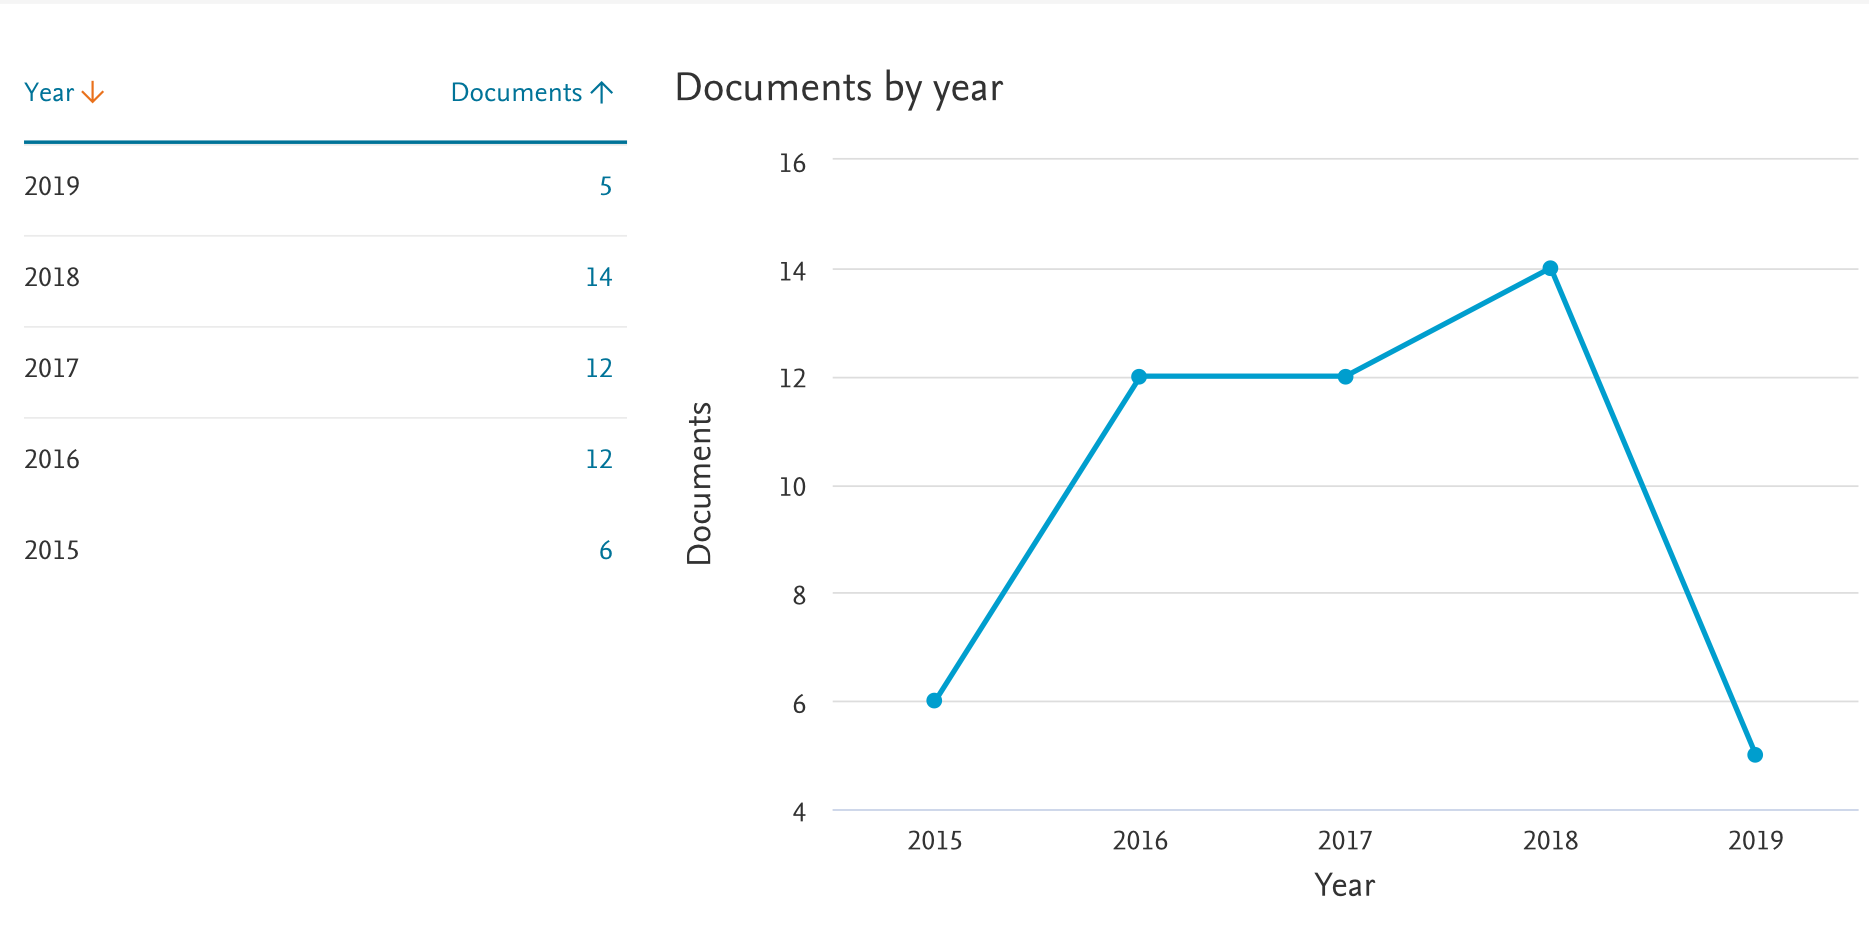
\includegraphics[width=\textwidth]{imagens/pubByYear.png}
	%\end{minipage}
\end{figure}

Para selecionar os artigos que ser\~{a}o abordados nessa pesquisa, foram verificados os t\'{i}tulos de cada artigo retornado pela \textit{query} pesquisada no Scopus que tivesse rela\c{c}\~{a}o direta com o t\'{o}pico desejado, passando pela leitura do resumo de cada um e encerrando com a verifica\c{c}\~{a}o da disponibilidade dos mesmos na base de dados da UNISINOS. Esta an\'{a}lise resultou na tabela:

% NOMEAR E REFERENCIAR TABELA %

\pagebreak
%\clearpage
%\newpage

\begin{table}[]
\begin{tabular}{|l|l|l|}
\hline
\textbf{Authors}                                                                                            & \textbf{Title}                                                                                                                                                       & \textbf{Year} \\ \hline
Fraser G.                                                                                                   & \begin{tabular}[c]{@{}l@{}}Gamification of software testing\end{tabular}                                                                                           & 2017          \\ \hline
\begin{tabular}[c]{@{}l@{}}De Jesus G.M., Ferrari F.C.,\\ De Paula Porto D., Fabbri S.C.P.F.\end{tabular}   & \begin{tabular}[c]{@{}l@{}}Gamification in software testing:\\ A characterization study\end{tabular}                                                               & 2018          \\ \hline
Elgrably I.S., Oliveira S.R.B.                                                                              & \begin{tabular}[c]{@{}l@{}}Gamification and evaluation of the use\\the agile tests in software quality\\subjects: The application of case\\studies\end{tabular} & 2018          \\ \hline
\begin{tabular}[c]{@{}l@{}}Pedreira O., García F., Brisaboa N.,\\ Piattini M.\end{tabular}                  & \begin{tabular}[c]{@{}l@{}}Gamification in software engineering -\\A systematic mapping\end{tabular}                                                              & 2015          \\ \hline
Houshmand M., Paydar S.                                                                                     & \begin{tabular}[c]{@{}l@{}}EMVille: A gamification-based\\approach to address the equivalent\\mutant problem\end{tabular}                                        & 2017          \\ \hline
Rojas J.M., Fraser G.                                                                                       & \begin{tabular}[c]{@{}l@{}}Code Defenders: A Mutation Testing\\Game\end{tabular}                                                                                    & 2016          \\ \hline
\end{tabular}
\end{table}

Na subseção ``discussão dos trabalhos'', os artigos filtrados ser\~{a}o abordados e analisados mais a fundo.

\subsection{Discussão dos trabalhos}
\cite{Fraser01} afirma que desenvolver bons testes de software é difícil e não é algo destacado no ensino da programação, além de não ser uma atividade que os desenvolvedores apreciam. O mesmo também destaca alguns aspectos importantes para bons testes, como a intuição humana, o entendimento de como o software deve funcionar e de qual o contexto do mesmo. Considerando os grandes problemas que podem ser causados por testes feitos de forma inadequada, o autor explica que seu artigo explora uma nova forma de resolver o problema dos testes: a gamificação. Com isso, quem já trabalha na área terá mais chances de se destacar, conhecendo novas ferramentas e técnicas de teste, além de facilitar o ensino nas escolas, onde o assunto é negligenciado quando se trata de programação. O autor também destaca o uso dessas ferramentas em \textit{crowdsourcing}, onde várias pessoas trabalham numa só finalidade. Ele finaliza descrevendo que a aplicação de gamificação tem potencial de melhorar a qualidade dos testes de software e, consequentemente, do software em geral. O autor também cita que as pesquisas no meio ainda estão num estágio bastante inicial, porém, já mostrou resultados promissores. Talvez, por não ter sido aplicado numa escala maior, ainda não há resultados concretos, porém, o autor poderia ter levantado alguns dados quantitativos relacionados ao experimento citado no quarto tópico do artigo.

\cite{DeJesus} apresentou um cenário geral de outros artigos que abordam gamificação nos testes de software, incluindo alguns dos artigos abordados aqui. O estudo foi dividido em seis categorias: contexto de aplicação, elementos de gamificação utilizados, objetivos da gamificação, técnicas de testes de software, níveis de teste e fases no processo de software. Considerando o contexto, os estudos eram focados em aplicações educacionais e industriais, sendo vários deles usados nos dois contextos; poucos eram exclusivos. Desses, os autores encontraram formas de aplicá-los em outros contextos. Por exemplo: um estudo que era focado no ambiente educacional sendo utilizado em ambientes industriais, e vice-versa. Sobre elementos de gamificação, os autores afirmam que a tríade PBL (\textit{Points, Badges, Leaderboard}, podendo ser traduzido como \textit{Pontos, Emblemas, Quadro de Líderes}) era a mais utilizada nos estudos, havendo apenas um estudo que não utilizou pontos e outro que não conseguiu aplicar sua metodologia no contexto correto. Entre os objetivos da gamificação, os autores apontam o maior desenvolvimento da criatividade, colaboração, engajamento, motivação e satisfação. Quanto às técnicas de teste, abordou-se a funcional, estrutural e baseados em falhas, sendo a última a mais utilizada nas aplicações de gamificação. Além disso, alguns estudos têm aplicabilidade nas três técnicas citadas. Nos níveis de teste, foram abordados os de unidade (dos quais a maioria são utilizados com outras ferramentas de automação), integração e de sistema. Aqui, os estudos tiveram foco nos testes de unidade. Os outros estudos não mencionaram em quais níveis eles poderiam ser aplicados, porém, os autores acreditam que a aplicabilidade é possível em todos os níveis citados. Quanto às fases no processo de software, os autores afirmam que praticamente todos os estudos podem ser aplicados em todo o processo, com exceção do planejamento e na configuração de dados e ambiente. Como sendo uma área nova na engenharia de software, os autores acreditam ser um tópico a ser monitorado quanto ao seu crescimento, especialmente na área de testes. 

\cite{Rojas} trouxe o desenvolvimento de um jogo chamado \textit{Code Defenders}, cujo objetivo é desenvolver e ensinar testes de mutantes. Ele funciona da seguinte forma: dois jogadores, sendo um atacante e um defensor, através da técnica de testes de mutantes, devem melhorar tanto seus casos de teste quanto o próprio código-fonte. No jogo, o atacante deve, propositalmente, introduzir uma falha numa classe Java (um mutante), e o defensor deve escrever um caso de teste no JUnit capaz de detectar esta falha (matar o mutante). O jogo funciona por rodadas de ataque e defesa, onde o primeiro a jogar é o atacante. Quando o atacante produz um mutante com sucesso, o defensor terá a chance de produzir uma defesa contra esse mutante. Caso o defensor consiga matar o mutante, ele leva um ponto; caso contrário, o atacante fica com um ponto. Se o mutante for equivalente, o \textit{gameplay} muda: se o defensor suspeita que este mutante é equivalente, o atacante é desafiado a aceitar essa suspeita, perdendo pontos e passando-os para o defensor, ou criar um caso de teste que mata este mutante; neste caso, cada jogador fica com um ponto. Alguns desafios citados pelos autores e que pode diminuir o alcance é que ele deve ter, obrigatoriamente, dois jogadores humanos, e que devem ter experiência com código em Java. É bem interessante a ideia do jogo, e abstrair a parte do código, fazendo metáforas com outras situações, é bastante promissor, e pode trazer ainda mais pessoas para a área, tanto de desenvolvimento quanto para testes.

\cite{Houshmand} traz um \textit{framework} para combater os mutantes equivalentes de forma eficiente. Os autores citam que testes de mutantes são muito custosos, e que quando os mesmos são equivalentes, trazem dificuldades de serem detectados pelos atacantes, fazendo o esforço não valer a pena. Alguns outros trabalhos foram citados pelos autores para atacar esse problema, como limitar algumas características do código desenvolvido para facilitar a detecção de mutantes, verificar padrões no código mutante, ou comparar os códigos originais com os mutantes no momento da compilação do código (também chamado de TCE). Concordando que mutantes não podem ser detectados sem interferência humana, os autores propõem um modelo de três camadas, em que primeira usa a técnica de TCE (sigla para \textit{Trivial Compiler Equivalence}, ou Equivalência do Compilador Trivial em português), a segunda usa a gamificação e a terceira pega os resultados das duas camadas e usa a técnica de \textit{machine-learning} para deixar a prática mais automatizada. A camada de gamificação se chamará \textit{EMVille}, em que especialistas entrarão em jornadas para resolver ou mitigar problemas de mutantes equivalentes. Porém, o método de pontuação não ficou claro, e não foi possível compreender de que formas o usuário irá pontuar, não pontuar ou, até mesmo, perder seus pontos. Além disso, na metáfora proposta para jogadores pouco familiarizados com o assunto, ficou bastante confuso, não parecendo ter relação com o problema que se está disposto a resolver. Porém, os autores afirmam que a proposta, testada num ambiente real, ajudou os profissionais a resolverem problemas de mutantes equivalentes.

\cite{Elgrably} mostra um estudo feito com estudantes de graduação e pós-graduação relacionado ao ensino de testes ágeis nas disciplinas de Qualidade de Software ensinadas nessas modalidades de ensino. A motivação dos autores é que o ensino de métodos ágeis só faz sentido para o aluno se ele viver aquilo na prática, e na vivência dos autores, o ensino apenas teórico desse tópico faz com que o aluno perca o interesse e o deixa despreparado para o mercado, em que os métodos ágeis estão em crescente uso. Como elementos de gamificação, os autores também utilizaram pontos, emblemas e quadro de líderes, além disso, dependendo do tipo da aula, foram usadas premiações, lista de desafios e narrativas. Outros elementos estavam presentes na pontuação dos alunos, como bônus pelo não-uso do celular, pela participação e frequência nas aulas. Porém, o mesmo não tem fundamentação teórica relacionada aos elementos de metodologia ágil utilizados no estudo deles, o que dificulta o entendimento de quem não faz parte dessa área de estudo. Mesmo assim, o estudo deles traz algo curioso: mesmo com maior participação e maior comunicação entre os alunos (o que foi apontado como algo bastante positivo), as notas dos mesmos diminuíram em relação às aulas convencionais. Nesse caso em específico, a gamificação trouxe uma dificuldade maior nas atividades e avaliou de forma diferente a participação dos alunos, como já mencionado. Por conta disso, os autores trouxeram a adaptação desse conteúdo para uso com a gamificação em sala de aula como um problema a ser resolvido, além de usar uma plataforma on-line para computar os pontos, entre outras melhorias. Contudo, o saldo foi positivo, e houve, sim, uma melhoria geral no ensino com o uso de gamificação.

%%%%%%%%% vou retirar do artigo %%%%%%%%%
% \cite{Parizi} trouxe um problema de rastreabilidade entre testes e o código-fonte, e propõe um \textit{framework} chamado GamiTracify para engajar e motivar os desenvolvedores nas tarefas de rastreabilidade. A ideia do autor é que quem desenvolve os testes incorporem (e mantenham, posteriormente) no código-fonte informações de rastreabilidade durante o desenvolvimento dos casos de teste, para evitar que as duas documentações fiquem dessincronizadas. Em comparação do uso desse \textit{framework} com uso de metodologias mais tradicionais apontaram uma melhoria nos links de rastreamento de qualidade. Entre os elementos de gamificação utilizados aqui estão os pontos, quadro de líderes, avatar e jornadas. Além da área de testes, este \textit{framework} também pode abranger as fases de desenvolvimento e manutenção, onde as informações de rastreabilidade são bastante úteis.

\cite{Pedreira} traz um panorama geral de gamificação no desenvolvimento de software. Aqui, é afirmado que, junto com as áreas de desenvolvimento e requisitos, a área de testes é bastante adequada para gamificação, visto que elas compartilham características como o nível de dificuldade em relação a outras tarefas do desenvolvimento de software, a necessidade de colaboração e, até mesmo, um alto índice de tédio. Nessas atividades, os autores afirmam que a gamificação ajuda bastante no rendimento, pois impulsiona o trabalho em equipe. Porém, mesmo considerando uma boa atividade para aplicação da gamificação, os autores não encontraram estudos muito completos na área de testes. Sobre elementos de gamificação, assim como foi apontado por \cite{DeJesus}, os mais utilizados foram os pontos, emblemas e quadro de líderes, além de também citar jornadas, como no trabalho de \cite{Houshmand}. Um aspecto importante apontado aqui é que a gamificação deve ser aplicada com cuidado na engenharia de software: muitos dos trabalhos estudados pelos autores falharam ao serem aplicados, justamente pela maioria deles usarem apenas o sistema de pontos, e ignorar muitos dos mecanismos de gamificação possíveis, levando muito rapidamente ao desuso devido à repetitividade. Um paralelo que pode ser feito é com o cenário cada vez maior de jogos on-line, em que as desenvolvedoras que não incrementam seus jogos e não criam eventos para incentivar seus jogadores, por exemplo, acabam por perder público. 

%%%%%%%%% vou retirar do artigo %%%%%%%%%
% \cite{Garcia} propuseram o GOAL (Gamification on Application Lifecycle Management), um \textit{framework} que possibilita aplicar a gamificação em qualquer fase do desenvolvimento de software. Os autores testaram o \textit{framework} numa empresa nas áreas de gerenciamento de requisitos, gestão de projetos e teste de software (onde foi mencionado apenas os testes unitários como objeto de estudo) e aplicaram os elementos de pontos, níveis, distintivos, quadro de líderes, gráfico social e desafio. O objetivo é de engajar usuários e melhorar seu desempenho, que foi alcançado, segundo os autores.


\section{Proposta inicial de metodologia}

% pensar no uso do jogo Code Defenders em conjunto com alguma outra metodologia.
% verificar último artigo que encontrei, na seção 3.2, e tentar adaptar com o cenário atual na empresa em que trabalho
% considerar o uso de alguma ferramenta de análise de código (como o Sonarqube) para avaliar o desempenho dos programadores envolvidos no processo e premiá-los de acordo com a índice de qualidade apontado pela ferramenta (e talvez aplicar isso nos códigos de testes automatizados tbm)
% pensar em como pontuar os programadores e testers pela cobertura de código: no caso dos programadores, o código deverá cobrir os requisitos, e no caso dos testers deverá cobrir os casos de teste (verificar ferramenta Hansel, que se integra com o JUnit)

% comentário do professor: Na metodologia, precisa apresentar as tarefas e um cronograma de como pretende desenvolver o trabalho em um semestre.

%=======================================================================
% Exemplos de Citações e Referências Bibliográficas
%=======================================================================

%=======================================================================
% Conclusão
%=======================================================================
\section{Conclusão}
Apesar de ser relativamente recente, a gamificação é um tema que está em constante crescimento na engenharia de software. Conforme observado, ela tem apresentado bons resultados, tanto na indústria quanto no ensino, e tem chegado no seu propósito de incentivar, motivar e melhorar o desempenho de funcionários, porém, a aplicação dessa metodologia em empresas reais aparenta ser bem difícil, principalmente em empresas maiores que já têm culturas e processos bem definidos. 

Em trabalhos futuros tem-se a ideia de aprofundar ainda mais no tema de gamificação, focando em todo o processo de testes de software, e elaborar um plano de aplicação dessa metodologia em empresas de pequeno porte, onde os processos ainda não estão bem definidos.

%=======================================================================
% Resumo em língua estrangeira (sim, é aqui mesmo).
%
% O idioma usado aqui deve necessariamente aparecer nos parâmetros do
% \documentclass, no início do documento.
%=======================================================================
\begin{otherlanguage}{english}
\othertitle{}
\begin{abstract}

\palavraschave{}
\end{abstract}
\end{otherlanguage}

%=======================================================================
% Referências
%=======================================================================
\bibliography{referencias}

%=======================================================================
% Exemplo de Apêndice
% O Apêndice é utilizado para apresentar material complementar elaborado
% pelo próprio autor.  Deve seguir as mesmas regras de formatação do
% corpo principal do documento.
%=======================================================================

%=======================================================================
% Exemplo de Anexo
% O Anexo é utilizado para a ``inclusão de materiais não elaborados pelo
% próprio autor, como cópias de artigos, manuais, folders, balancetes, etc.
% e não precisam estar em conformidade com o modelo''.
%=======================================================================

\end{document}
